\subsection{NoScript f�r Mozilla Firefox}
Die Einstellungen f�r JavaScript lassen sich mit dem Add-on \textit{NoScript} komfortabel verwalten. Die Erweiterung kann von der Website \footnote{ \href{https://addons.mozilla.org/de/firefox/addon/noscript/}{https://addons.mozilla.org/de/firefox/addon/noscript}} installiert werden. Ein einfacher Klick auf das Download-Symbol startet die Installation. Im Anschluss ist Firefox neu zu starten.\\

\begin{figure}[htb]
\begin{center}
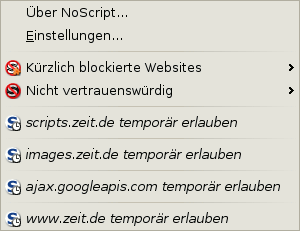
\includegraphics[scale=0.75]{../screenshots/noscript_allow.png}
\caption{NoScript-Button und Men� in der Statuszeile}
\label{abb:noscript_button}
\end{center}
\end{figure}

Nach dem Neustart von Firefox ist in der Statusleiste ein zus�tzliches Symbol vorhanden, welches den Status der Freigabe von JavaScript anzeigt. Ein Klick auf das Symbol �ffnet das im Bild \ref{abb:noscript_button} gezeigte Men�, welches JavaScript f�r die aktuellen Sites generell oder nur tempor�r freigibt.\\

Einige Webseiten verwenden \textit{Captchas} als Spamschutz. Die Captchas werden von Drittseiten eingebunden (Recaptcha.com, Nucaptcha.com...) und funktionieren nur, wenn Javascript f�r den Captcha-Provider freigegeben ist. Wenn das Captcha auf einer Webseite nicht funktioniert, schauen sie in der NoScript-Liste nach, ob evtl. ein Captcha-Provider dabei ist und geben sie Javascript tempor�r f�r diese Domain frei.\\

Weitere Skripte von Drittanbietern werden �blicherweise nur zum Spionieren verwendet und sind f�r die Funktionalit�t selten notwendig.\\

W�hlt man den Punkt \textit{Einstellungen} im NoScript-Men�, �ffnet sich der Einstellungsdialog (Bild \ref{abb:noscript_einst}), der auf dem Reiter \textit{Positivliste} eine Liste der Websites zeigt, f�r welche Java-Script freigegeben wurde. Als Erstes sollte man aus der Positivliste alles entfernen, was man nicht wirklich braucht. In der Liste findet man standardm��ig mit \textit{googlesyndications} auch Surf-Tracker.\\

\begin{figure}[htb]
\begin{center}
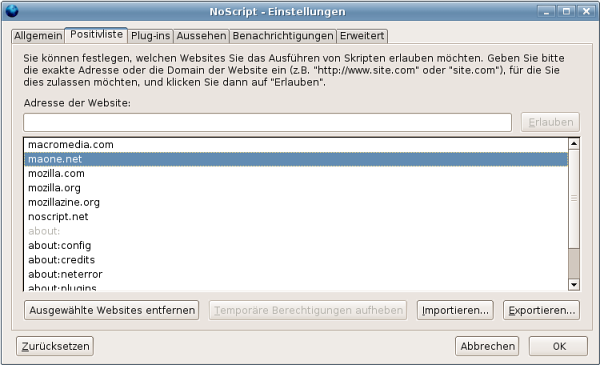
\includegraphics[scale=0.58]{../screenshots/noscript_einst.png}
\caption{Einstellungen f�r NoScript}
\label{abb:noscript_einst}
\end{center}
\end{figure}

Auf dem Reiter \textit{Benachrichtigungen} l�sst sich beispielsweise konfigurieren, ob NoScript den Surfer mit einem Sound oder mit einem Info-Balken dar�ber informiert, dass Scripte auf der aktuellen Webseite blockiert wurden.\\

Der Sound nervt mich, diese Option habe ich deaktiviert. Wenn eine Webseite jedoch nicht wie erwartet funktioniert, kann die kurze Einblendung eines Info-Balkens hilfreich bei der Suche nach den Ursachen sein.\\

NoScript dient nicht nur der Steuerung von Javascript, es bieten \textbf{Schutz gegen vielf�ltige Angriffe} aus dem Netz. (XSS-Angriffe, Webbugs, Click-Hijacking....). Au�erdem blockiert es auch Ping-Attribute und kann f�r eine LIste von Webseiten SSL-Verschl�sselung erzwingen. 
